% !TeX program = xelatex
\documentclass[a4paper,10pt]{article}

% ============================================================================
% សន្លឹកកិច្ចការសិស្ស ស-ខ្មៅ (Student Fill-In Worksheet — No-LCD Classroom)
% មេរៀនទី១៧ (១៧.២)៖ ការគណនាមាឌនៃព្រីស (ត្រូវគ្នា ១០០% នឹង LS_Plan_PRISM_VOL.tex)
% ============================================================================
\usepackage[a4paper, left=0.95cm, right=0.95cm, top=0.75cm, bottom=0.90cm, footskip=0.48cm]{geometry}
\usepackage{amsmath}
\usepackage{unicode-math}
\usepackage{fontspec}
\usepackage{array, colortbl}
\usepackage[table]{xcolor}
\usepackage{enumitem}
\usepackage{pifont}
\usepackage{fancyhdr}
\usepackage{lastpage}
\usepackage{tikz}
\usepackage[most]{tcolorbox}
\usetikzlibrary{calc, arrows.meta, angles, quotes, patterns, decorations.markings, babel}

\makeatletter
\let\@expl@@@mark@update@singlecol@structures@@\relax
\makeatother

\providecommand{\NGSFindFonts}{%
  \IfFileExists{C:/Windows/Fonts/cambria.ttc}{%
    \def\NGSSysPath{C:/Windows/Fonts/}%
    \def\NGSUserPath{C:/Users/KIT/AppData/Local/Microsoft/Windows/Fonts/}%
  }{%
    \IfFileExists{./fonts/KhmerOSsiemreap.ttf}{\def\NGSSysPath{./fonts/}\def\NGSUserPath{./fonts/}}{%
    \IfFileExists{../fonts/KhmerOSsiemreap.ttf}{\def\NGSSysPath{../fonts/}\def\NGSUserPath{../fonts/}}{%
    \IfFileExists{../../fonts/KhmerOSsiemreap.ttf}{\def\NGSSysPath{../../fonts/}\def\NGSUserPath{../../fonts/}}{%
    \IfFileExists{../../../fonts/KhmerOSsiemreap.ttf}{\def\NGSSysPath{../../../fonts/}\def\NGSUserPath{../../../fonts/}}{%
    \IfFileExists{../../../../fonts/KhmerOSsiemreap.ttf}{\def\NGSSysPath{../../../../fonts/}\def\NGSUserPath{../../../../fonts/}}{%
    \IfFileExists{../../../../../fonts/KhmerOSsiemreap.ttf}{\def\NGSSysPath{../../../../../fonts/}\def\NGSUserPath{../../../../../fonts/}}{%
    \IfFileExists{../../../../../../fonts/KhmerOSsiemreap.ttf}{\def\NGSSysPath{../../../../../../fonts/}\def\NGSUserPath{../../../../../../fonts/}}{%
      \def\NGSSysPath{../../../../../../../fonts/}\def\NGSUserPath{../../../../../../../fonts/}%
    }}}}}}}%
  }%
}
\NGSFindFonts

\setmathfont[Path={\NGSSysPath}, FontIndex=1, Scale=1.02]{cambria.ttc}
\defaultfontfeatures{Ligatures=TeX}

\setmainfont[
  Path={\NGSUserPath},
  Extension=.ttf,
  Script=Khmer,
  BoldFont={KhmerOSsiemreap},
  BoldFeatures={FakeBold=1.8},
  ItalicFont={KhmerOSsiemreap},
  ItalicFeatures={FakeSlant=0.25},
  BoldItalicFont={KhmerOSsiemreap},
  BoldItalicFeatures={FakeBold=1.8, FakeSlant=0.25}
]{KhmerOSsiemreap}

\newfontfamily\muol[Path={\NGSUserPath}, Extension=.ttf, Script=Khmer]{KhmerOSmuollight}
\newfontfamily\TimesEn[Path={\NGSSysPath}, Extension=.ttf, BoldFont={timesbd}, ItalicFont={timesi}, BoldItalicFont={timesbi}]{times}

\XeTeXlinebreaklocale "km"
\XeTeXlinebreakskip = 0pt plus 1pt minus 0.1pt

\definecolor{panelgray}{gray}{0.93}
\definecolor{headgray}{gray}{0.85}

\pagestyle{fancy}
\fancyhf{}
\renewcommand{\headrulewidth}{0pt}
\fancyfoot[L]{\fontsize{8pt}{10pt}\selectfont អនុវិទ្យាល័យព្រះក្រសាំង \en{---} គណិតវិទ្យា ថ្នាក់ទី៨ \en{|} មេរៀនទី១៧ (១៧.២ ការគណនាមាឌនៃព្រីស)}
\fancyfoot[R]{\fontsize{8.2pt}{10pt}\selectfont ទំព័រ \en{\thepage\ / \pageref{LastPage}}}

\setlength{\parindent}{0pt}
\setlength{\parskip}{0pt}
\setlength{\tabcolsep}{4pt}

\newcommand{\en}[1]{{\TimesEn #1}}
\newcommand{\enbf}[1]{{\TimesEn\textbf{#1}}}
\newcommand{\unit}[1]{\,\text{\en{#1}}}
\newcommand{\cnum}[1]{\mbox{\fontsize{10pt}{12pt}\selectfont\ding{\numexpr181+#1\relax}}}
\newcommand{\chkbox}{\tikz[baseline=-0.15ex]\draw[black, line width=0.85pt] (0,0) rectangle (0.25cm,0.25cm);}
\newcommand{\blank}[1]{\makebox[#1]{\dotfill}}
\newcommand{\tri}[1]{\ensuremath{\triangle #1}}

\newcommand{\rightbox}[4][0.18]{%
  \draw[black, line width=0.8pt]
    ($(#3)!#1!(#2)$) -- ($($(#3)!#1!(#2)$)+($(#3)!#1!(#4)$)-(#3)$) -- ($(#3)!#1!(#4)$);
}

\newcommand{\secbar}[2]{%
  \vspace{3pt}%
  \begin{tcolorbox}[
    enhanced, sharp corners, colback=headgray, colframe=black,
    boxrule=0.9pt, boxsep=1pt, top=2.5pt, bottom=2.5pt, left=6pt, right=6pt,
    after skip=3pt
  ]
    {\muol\fontsize{9.2pt}{13.5pt}\selectfont #1}\hfill{\fontsize{8.3pt}{11.5pt}\selectfont\textbf{#2}}
  \end{tcolorbox}%
}

\newcolumntype{L}[1]{>{\raggedright\arraybackslash}p{#1}}
\newcolumntype{C}[1]{>{\centering\arraybackslash}p{#1}}

\begin{document}
\fontsize{9.4pt}{13.8pt}\selectfont

% ============================================================================
% ទំព័រទី ១៖ ក្បាលសន្លឹកកិច្ចការ + E1 (POE Overflow) + E2 (ស្រទាប់គូបឯកតា & គំរូទី 1, 2) + E3 (រូបមន្ត)
% ============================================================================
\begin{tcolorbox}[
  enhanced, sharp corners, colback=white, colframe=black,
  boxrule=1.1pt, boxsep=2.5pt, top=6pt, bottom=6pt, left=6pt, right=6pt, after skip=8pt
]
  \begin{center}
    {\muol\fontsize{10pt}{14.5pt}\selectfont សន្លឹកកិច្ចការសិស្ស \enbf{---} គណិតវិទ្យា ថ្នាក់ទី៨ \enbf{(}១៧\enbf{.}២ ការគណនាមាឌនៃព្រីស\enbf{)}}\\[3.5pt]
    {\fontsize{8.8pt}{12pt}\selectfont
    ឈ្មោះសិស្ស / ដៃគូ៖ \blank{6.2cm} \hspace{0.2cm}
    ថ្នាក់៖ \blank{1.4cm} \hspace{0.2cm}
    ក្រុម៖ \blank{1.2cm} \hspace{0.2cm}
    កាលបរិច្ឆេទ៖ \blank{2.8cm}}
  \end{center}
\end{tcolorbox}

% --- E1 Engage: POE Water Overflow Mystery (Ex #15 p. 229) ---
\begin{tcolorbox}[
  enhanced, sharp corners, colback=panelgray, colframe=black,
  boxrule=0.8pt, boxsep=2.5pt, top=6pt, bottom=6pt, left=6pt, right=6pt, after skip=8pt
]
  \textbf{បេសកកម្មទី១ (\en{E1 - Engage / POE})៖ ចាក់ទឹកពីពែងស៊ីឡាំងចូលថាសប្រអប់កែង — ហៀរ ឬមិនហៀរ?}\\[3pt]
  គេដងទឹកពេញពែងរាងស៊ីឡាំងមួយដែលមានអង្កត់ផ្ចិតបាត $d = 8\unit{cm}$ និងកម្ពស់ $h = 15\unit{cm}$ រួចចាក់ទឹកនោះទាំងអស់ចូលទៅក្នុងថាសប្រអប់កែងទទេមួយមានទំហំ $15\unit{cm}\times 10\unit{cm}\times 5\unit{cm}$ (លំហាត់ទី១៥ ទំព័រ ២២៩) ។\\[3pt]
  \ding{226}\ ទស្សន៍ទាយជាដៃគូមុនគណនា៖ \;\chkbox\ ទឹកមិនពេញថាសទេ \hspace{0.45cm} \chkbox\ ទឹកពេញថាសល្មម \hspace{0.45cm} \chkbox\ ទឹកហៀរចេញក្រៅថាស!
\end{tcolorbox}

% --- E2 Explore Part A: 3-Layer Unit-Cube Structuring (p. 222) ---
\secbar{ផ្នែកទី១ \enbf{(}ក\enbf{)} ៖ ការរាប់ស្រទាប់គូបឯកតា $1\unit{cm}^3$ ដើម្បីទាញរករូបមន្តមាឌព្រីស \enbf{(E2 - Explore)}}{ការងារជាដៃគូ \en{5 min}}

\noindent
\begin{minipage}[c]{8.3cm}
  \centering
  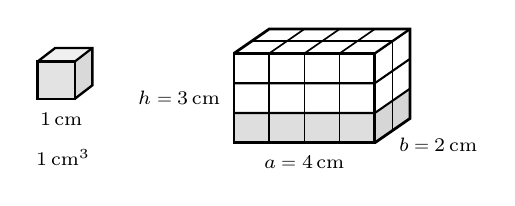
\begin{tikzpicture}[scale=0.86, every node/.style={font=\scriptsize, text=black}]
    % (1) គូបឯកតា 1 cm^3
    \begin{scope}[shift={(-3.55,0.20)}]
      \fill[gray!22] (0,0) rectangle (0.55,0.55);
      \fill[gray!12] (0,0.55) -- (0.26,0.75) -- (0.81,0.75) -- (0.55,0.55) -- cycle;
      \fill[gray!30] (0.55,0) -- (0.81,0.20) -- (0.81,0.75) -- (0.55,0.55) -- cycle;
      \draw[black, line width=0.85pt] (0,0) rectangle (0.55,0.55);
      \draw[black, line width=0.85pt] (0,0.55) -- (0.26,0.75) -- (0.81,0.75) -- (0.81,0.20) -- (0.55,0);
      \draw[black, line width=0.8pt] (0.55,0.55) -- (0.81,0.75);
      \node[below=1pt] at (0.35,-0.02) {$1\unit{cm}$};
      \node[align=center] at (0.38,-0.82) {\textbf{គូបឯកតា}\\$1\unit{cm}^3$};
    \end{scope}

    % (2) ប្រអប់កែង 4 x 2 x 3 cm (3 ស្រទាប់)
    \begin{scope}[shift={(-0.65,-0.45)}]
      \def\ux{0.52}
      \def\uy{0.44}
      \def\sx{0.26}
      \def\sy{0.18}
      \fill[gray!26] (0,0) rectangle (4*\ux,\uy);
      \fill[gray!32] (4*\ux,0) -- ($(4*\ux+2*\sx,2*\sy)$) -- ($(4*\ux+2*\sx,\uy+2*\sy)$) -- (4*\ux,\uy) -- cycle;
      \foreach \x in {1,2,3} {
        \draw[black, line width=0.6pt] (\x*\ux,0) -- (\x*\ux,3*\uy);
        \draw[black, line width=0.6pt] (\x*\ux,3*\uy) -- ($(\x*\ux+2*\sx,3*\uy+2*\sy)$);
      }
      \foreach \y in {1,2} {
        \draw[black, line width=0.75pt] (0,\y*\uy) -- (4*\ux,\y*\uy) -- ($(4*\ux+2*\sx,\y*\uy+2*\sy)$);
      }
      \draw[black, line width=0.6pt] (\sx,3*\uy+\sy) -- ($(4*\ux+\sx,3*\uy+\sy)$) -- ($(4*\ux+\sx,\sy)$);
      \draw[black, line width=1.0pt] (0,0) rectangle (4*\ux,3*\uy);
      \draw[black, line width=1.0pt] (0,3*\uy) -- ($(2*\sx,3*\uy+2*\sy)$) -- ($(4*\ux+2*\sx,3*\uy+2*\sy)$) -- ($(4*\ux+2*\sx,2*\sy)$) -- (4*\ux,0);
      \draw[black, line width=0.85pt] (4*\ux,3*\uy) -- ($(4*\ux+2*\sx,3*\uy+2*\sy)$);
      \node[below=1pt] at (2*\ux,0) {$a = 4\unit{cm}$};
      \node[below right=-1pt] at ($(4*\ux+\sx,\sy)$) {$b = 2\unit{cm}$};
      \node[left=1.5pt] at (0,1.5*\uy) {$h = 3\unit{cm}$};
    \end{scope}
  \end{tikzpicture}
\end{minipage}%
\hfill
\begin{minipage}[c]{10.3cm}\raggedright
  \textbf{ពិនិត្យរូបប្រអប់កែងទំហំ $4\unit{cm}\times 2\unit{cm}\times 3\unit{cm}$ (ទំ.២២២)៖}\\[6pt]
  $1.$ ស្រទាប់បាត ១ មានគូបឯកតាចំនួន៖ $4 \times 2 = \mathbf{\blank{1.1cm}}$ គូប\\
  \hspace*{0.3cm}\textit{(ត្រូវនឹងតម្លៃលេខនៃផ្ទៃក្រឡាបាត $B = a\times b = \blank{1.1cm}\unit{cm}^2$)} ។\\[5.5pt]
  $2.$ ប្រអប់ទាំងមូលមានកម្ពស់ $h = 3$ ស្រទាប់បន្តុបលើគ្នា៖\\
  \hspace*{0.3cm}ចំនួនគូបសរុប $= \blank{1.0cm}\text{ គូប/ស្រទាប់} \times 3\text{ ស្រទាប់} = \mathbf{\blank{1.2cm}}\unit{cm}^3$ ។\\[5.5pt]
  $3.$ ជាទូទៅ ចំពោះគ្រប់ព្រីសត្រង់មានផ្ទៃក្រឡាបាត $B$ និងកម្ពស់ $h$៖\\
  \hspace*{0.3cm}មាឌនៃព្រីស៖ $V = \text{ផ្ទៃក្រឡាបាត} \times \text{កម្ពស់} = \mathbf{\blank{1.8cm}}$ ។
\end{minipage}

\vspace{18pt}
% --- E2 Explore Part B: Worked Examples 1 & 2 (p. 223) ---
\secbar{ផ្នែកទី១ \enbf{(}ខ\enbf{)} ៖ អនុវត្តលំហាត់គំរូទី \enbf{1} និងទី \enbf{2 (}ទំព័រ ២២៣ \enbf{---} ប្រយ័ត្នព្រីសដេកផ្ដេក\enbf{!)}}{ការងារជាដៃគូ \en{6 min}}

\noindent
\begin{minipage}[t]{8.6cm}\vspace{0pt}
  \begin{tcolorbox}[
    enhanced, sharp corners, colback=white, colframe=black, equal height group=rowEx12,
    boxrule=0.8pt, boxsep=3pt, top=7.5pt, bottom=7.5pt, left=5pt, right=5pt
  ]\raggedright
    \textbf{គំរូទី \en{1} (ទំ.២២៣)៖ ព្រីសចតុមុខកែង $20\times 5\times 15$}\\[6.5pt]
    $1.$ ផ្ទៃក្រឡាបាតចតុមុខកែង៖\\
    \hspace*{0.2cm}$B = a \times b = 20 \times 5 = \blank{1.4cm}$ ឯកតាផ្ទៃ\\[6.5pt]
    $2.$ កម្ពស់នៃព្រីស៖ $h = 15$\\[6.5pt]
    $3.$ មាឌនៃព្រីស៖\\
    \hspace*{0.2cm}$V = B \cdot h = \blank{1.3cm} \times 15 = \blank{1.5cm}$ ឯកតាមាឌ ។
  \end{tcolorbox}
\end{minipage}%
\hfill
\begin{minipage}[t]{10.1cm}\vspace{0pt}
  \begin{tcolorbox}[
    enhanced, sharp corners, colback=white, colframe=black, equal height group=rowEx12,
    boxrule=0.8pt, boxsep=3pt, top=7.5pt, bottom=7.5pt, left=5pt, right=5pt
  ]
    \textbf{គំរូទី \en{2} (ទំ.២២៣)៖ ព្រីសត្រីកោណសមបាទដេកផ្ដេក ($10, 10, 12$; ប្រវែង $15$)}\\[5pt]
    \begin{minipage}[c]{6.3cm}\raggedright
      $1.$ បាតជាត្រីកោណសមបាទ (បាត $12$, ជ្រុង $10$)៖\\[4.5pt]
      $\bullet$ កម្ពស់ត្រីកោណបាត (តាមពីតាករ)៖\\
      \hspace*{0.15cm}$h_{\tri{}} = \sqrt{10^2 - 6^2} = \sqrt{\blank{1.1cm}} = \blank{1.0cm}$\\[4.5pt]
      $\bullet$ ផ្ទៃបាត៖ $B = \dfrac{1}{2}\times 12\times \blank{0.9cm} = \blank{1.1cm}$\\[4.5pt]
      $2.$ មាឌព្រីស ($h = 15$)៖\\
      \hspace*{0.15cm}$V = B\cdot h = \blank{1.0cm}\times 15 = \blank{1.3cm}$ ឯកតាមាឌ ។
    \end{minipage}%
    \hfill
    \begin{minipage}[c]{2.8cm}
      \centering
      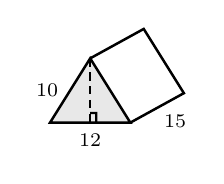
\begin{tikzpicture}[scale=0.68, every node/.style={font=\scriptsize, text=black}]
        \coordinate (P1) at (-1.25,-0.65);
        \coordinate (P2) at (0.25,-0.65);
        \coordinate (P3) at (-0.50,0.55);
        \coordinate (M) at (-0.50,-0.65);
        \coordinate (Q2) at (1.25,-0.10);
        \coordinate (Q3) at (0.50,1.10);
        \fill[gray!18] (P1) -- (P2) -- (P3) -- cycle;
        \draw[black, line width=0.9pt] (P1) -- (P2) -- (P3) -- cycle (P2) -- (Q2) -- (Q3) -- (P3);
        \draw[black, line width=0.75pt, densely dashed] (P3) -- (M);
        \rightbox[0.15]{P3}{M}{P2}
        \node[below=0.5pt] at (-0.50,-0.65) {$12$};
        \node[left=0.5pt] at ($0.5*(P1)+0.5*(P3)$) {$10$};
        \node[below right=-1pt] at ($0.5*(P2)+0.5*(Q2)$) {$15$};
      \end{tikzpicture}
    \end{minipage}
  \end{tcolorbox}
\end{minipage}

\vspace{18pt}
% --- E3 Explain: Formula Summary & Orientation Guard ---
\secbar{ផ្នែកទី២ ៖ សង្ខេបរូបមន្តមាឌនៃព្រីស ស៊ីឡាំង និងការសម្គាល់មុខបាត \enbf{(E3 - Explain)}}{សង្ខេបរួមគ្នា \en{6 min}}

\begin{tcolorbox}[
  enhanced, sharp corners, colback=white, colframe=black,
  boxrule=0.9pt, boxsep=4.5pt, top=9.5pt, bottom=9.5pt, left=6pt, right=6pt
]
  {\renewcommand{\arraystretch}{2.05}\footnotesize
  \begin{tabular}{|L{4.70cm}|L{5.80cm}|L{6.60cm}|}
    \hline
    \cellcolor{headgray}\textbf{ប្រភេទសូលីត} & \cellcolor{headgray}\textbf{រូបមន្តគណនាមាឌ ($V$)} & \cellcolor{headgray}\textbf{របៀបកំណត់មុខបាត $B$ និងកម្ពស់ $h$} \\
    \hline
    $1.$ ព្រីសត្រង់ទូទៅ (ត្រីមុខ, ចតុមុខ...) & $V = \blank{1.0cm} \times \blank{1.0cm}$ & $B =$ ផ្ទៃមុខពហុកោណពីរដែលប៉ុនគ្នានិងស្របគ្នា \\
    \hline
    $2.$ ប្រអប់កែង និង គូប & ប្រអប់កែង៖ $V = a\cdot b\cdot h$ \;\textbar\; គូប៖ $V = \blank{1.1cm}$ & គុណវិមាត្រទាំងបីដែលមានខ្នាតរង្វាស់ដូចគ្នា \\
    \hline
    $3.$ ស៊ីឡាំងបរិវត្ត (បាតជាថាសកាំ $r$) & $V = B\cdot h = \pi \times \blank{0.9cm} \times h$ & បើប្រាប់អង្កត់ផ្ចិត $d$ ត្រូវរកកាំ $r = \dfrac{d}{2}$ ជាមុន! \\
    \hline
  \end{tabular}}\\[9.5pt]
  $\bullet$ \textbf{ខ្នាតមាឌ និងចំណុះ៖}
  $1\unit{cm}^3 = 1000\unit{mm}^3$ \;\textbar\;
  $1\unit{dm}^3 = 1\unit{L}\text{ (លីត្រ)} = 1000\unit{cm}^3$ \;\textbar\;
  $1\unit{m}^3 = 1000\unit{dm}^3$\\[7.5pt]
  $\bullet$ \textbf{ធនាគារហេតុផល៖}
  \cnum{1} បាត $B$ ជាមុខពីរប៉ុនគ្នានិងស្របគ្នា \;\textbar\;
  \cnum{2} $h$ ជាចម្ងាយកែងរវាងបាតទាំងពីរ \;\textbar\;
  \cnum{3} $V = B\cdot h$ \;\textbar\;
  \cnum{4} ខ្នាតគូប ($\unit{cm}^3, \unit{m}^3$)
\end{tcolorbox}

\newpage

% ============================================================================
% ទំព័រទី ២៖ E4 (ប្រតិបត្តិ ក និង ខ ទំ.២២៣) + E5 (បកស្រាយបេសកកម្មទី១៥ & Exit Check) + កិច្ចការផ្ទះ
% ============================================================================

\secbar{ផ្នែកទី៣ ៖ អនុវត្តលំហាត់ប្រតិបត្តិ ក និង ខ ទំព័រ ២២៣ \enbf{(E4 - Elaborate)}}{អនុវត្ត \en{10 min}}

\noindent
\begin{minipage}[t]{9.1cm}\vspace{0pt}
  \begin{tcolorbox}[
    enhanced, sharp corners, colback=white, colframe=black, equal height group=rowE4,
    boxrule=0.85pt, boxsep=3.5pt, top=7pt, bottom=7pt, left=5.5pt, right=5.5pt
  ]\raggedright
    \textbf{៣.ក ប្រតិបត្តិ ក (ទំ.២២៣)៖ ព្រីសចតុមុខកែង}\\
    គណនាមាឌនៃព្រីសចតុមុខកែងខាងក្រោម៖
    \begin{center}
      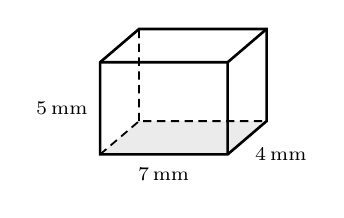
\begin{tikzpicture}[scale=0.90, every node/.style={font=\scriptsize, text=black}]
        \coordinate (A) at (-1.20,-0.65);
        \coordinate (B) at (0.60,-0.65);
        \coordinate (C) at (1.15,-0.18);
        \coordinate (D) at (-0.65,-0.18);
        \coordinate (A1) at (-1.20,0.65);
        \coordinate (B1) at (0.60,0.65);
        \coordinate (C1) at (1.15,1.12);
        \coordinate (D1) at (-0.65,1.12);
        \fill[gray!16] (A) -- (B) -- (C) -- (D) -- cycle;
        \draw[black, line width=0.95pt] (A) -- (B) -- (C) -- (C1) -- (D1) -- (A1) -- cycle;
        \draw[black, line width=0.95pt] (A1) -- (B1) -- (C1) (B) -- (B1);
        \draw[black, line width=0.65pt, densely dashed] (A) -- (D) -- (C) (D) -- (D1);
        \node[below=1pt] at (-0.30,-0.65) {$7\unit{mm}$};
        \node[below right=-1pt] at (0.90,-0.45) {$4\unit{mm}$};
        \node[left=1pt] at (-1.20,0.0) {$5\unit{mm}$};
      \end{tikzpicture}
    \end{center}
    $1.$ ផ្ទៃក្រឡាបាតចតុមុខកែង៖\\[4pt]
    \hspace*{0.2cm}$B = 4 \times 7 = \blank{1.4cm}\unit{mm}^2$\\[6pt]
    $2.$ កម្ពស់នៃព្រីស៖ $h = \blank{1.2cm}\unit{mm}$\\[6pt]
    $3.$ មាឌនៃព្រីស៖ $V = B \cdot h = \blank{1.2cm} \times \blank{1.0cm} = \blank{1.5cm}\unit{mm}^3$
  \end{tcolorbox}
\end{minipage}%
\hfill
\begin{minipage}[t]{9.7cm}\vspace{0pt}
  \begin{tcolorbox}[
    enhanced, sharp corners, colback=white, colframe=black, equal height group=rowE4,
    boxrule=0.85pt, boxsep=3.5pt, top=7pt, bottom=7pt, left=5.5pt, right=5.5pt
  ]\raggedright
    \textbf{៣.ខ ប្រតិបត្តិ ខ (ទំ.២២៣)៖ ព្រីសត្រីកោណកែងដេកផ្ដេក}\\
    គូសឆ្នូតស្រមោលលើមុខបាតត្រីកោណ រួចគណនាមាឌ៖
    \begin{center}
      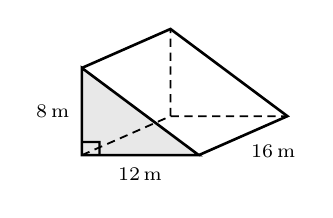
\begin{tikzpicture}[scale=0.90, every node/.style={font=\scriptsize, text=black}]
        \coordinate (A) at (-1.40,-0.65);
        \coordinate (B) at (0.25,-0.65);
        \coordinate (C) at (-1.40,0.58);
        \coordinate (A2) at (-0.15,-0.10);
        \coordinate (B2) at (1.50,-0.10);
        \coordinate (C2) at (-0.15,1.13);
        \fill[gray!18] (A) -- (B) -- (C) -- cycle;
        \draw[black, line width=0.95pt] (A) -- (B) -- (C) -- cycle;
        \draw[black, line width=0.95pt] (B) -- (B2) -- (C2) -- (C);
        \draw[black, line width=0.65pt, densely dashed] (A) -- (A2) -- (B2) (A2) -- (C2);
        \rightbox[0.15]{C}{A}{B}
        \node[left=1pt] at (-1.40,-0.03) {$8\unit{m}$};
        \node[below=1pt] at (-0.58,-0.65) {$12\unit{m}$};
        \node[below right=-1pt] at (0.90,-0.40) {$16\unit{m}$};
      \end{tikzpicture}
    \end{center}
    $1.$ មុខបាតជាត្រីកោណកែងជើង $8\unit{m}$ និង $12\unit{m}$៖\\
    \hspace*{0.2cm}$B = \dfrac{1}{2}\times \blank{0.9cm}\times \blank{0.9cm} = \blank{1.3cm}\unit{m}^2$\\[5.5pt]
    $2.$ ចម្ងាយកែងរវាងបាតត្រីកោណទាំងពីរ៖ $h = \blank{1.2cm}\unit{m}$\\[5.5pt]
    $3.$ មាឌនៃព្រីស៖ $V = B\cdot h = \blank{1.1cm}\times \blank{1.1cm} = \blank{1.5cm}\unit{m}^3$
  \end{tcolorbox}
\end{minipage}

\vspace{16pt}
% --- E5 Evaluate: Resolve E1 Water Overflow (Ex #15 p. 229) + Exit Check ---
\secbar{ផ្នែកទី៤ ៖ វាយតម្លៃ \enbf{---} បកស្រាយបេសកកម្ម \enbf{E1 (}លំហាត់ទី១៥ ទំ\enbf{.}២២៩\enbf{)} និង \enbf{Exit Check (E5)}}{ធ្វើដោយឯករាជ្យ \en{10 min}}

\noindent
\begin{minipage}[t]{10.2cm}\vspace{0pt}
  \begin{tcolorbox}[
    enhanced, sharp corners, colback=white, colframe=black, equal height group=rowE5,
    boxrule=0.85pt, boxsep=3.5pt, top=8pt, bottom=8pt, left=5.5pt, right=5.5pt
  ]\raggedright
    \textbf{៤.ក បកស្រាយបេសកកម្មទី១ — លំហាត់ទី១៥ (ទំ.២២៩, $\pi\approx 3.14$)៖}\\[6.5pt]
    $1.$ \textbf{មាឌទឹកពេញពែងរាងស៊ីឡាំង} ($d = 8\unit{cm} \Rightarrow r = \blank{0.9cm}\unit{cm},\; h = 15\unit{cm}$)៖\\[4.5pt]
    \hspace*{0.15cm}$V_{\text{ពែង}} = \pi r^2 h \approx 3.14 \times (\blank{0.8cm})^2 \times 15 = 3.14 \times \blank{1.1cm} = \blank{1.5cm}\unit{cm}^3$\\[7pt]
    $2.$ \textbf{មាឌថាសប្រអប់កែងទទេ} ($15\unit{cm}\times 10\unit{cm}\times 5\unit{cm}$)៖\\[4.5pt]
    \hspace*{0.15cm}$V_{\text{ថាស}} = 15 \times 10 \times 5 = \blank{1.6cm}\unit{cm}^3$\\[7pt]
    $3.$ \textbf{ប្រៀបធៀប និងសន្និដ្ឋាន៖} ដោយ $V_{\text{ពែង}}$ \blank{0.8cm} $V_{\text{ថាស}}$ ($>$ ឬ $<$)\\[4.5pt]
    \hspace*{0.15cm}ដូចនេះ៖ \;\chkbox\ \textbf{ទឹកមិនហៀរទេ} \hspace{0.5cm} \chkbox\ \textbf{ទឹកហៀរចេញក្រៅថាស!}
  \end{tcolorbox}
\end{minipage}%
\hfill
\begin{minipage}[t]{8.6cm}\vspace{0pt}
  \begin{tcolorbox}[
    enhanced, sharp corners, colback=white, colframe=black, equal height group=rowE5,
    boxrule=0.85pt, boxsep=3.5pt, top=8pt, bottom=8pt, left=5.5pt, right=5.5pt
  ]\raggedright
    \textbf{៤.ខ សំណួរត្រួតពិនិត្យរហ័ស (\en{Exit Check})៖}\\
    គូសវង់ជុំវិញអក្សរនៃចម្លើយត្រឹមត្រូវតែមួយគត់៖\\[7.5pt]
    \textbf{សំណួរទី១៖} រូបមន្តគណនាមាឌនៃព្រីសត្រង់ទូទៅគឺ៖\\[3pt]
    \hspace*{0.15cm}\textbf{ក.} $V = P \cdot h$ \hspace{0.55cm} \textbf{ខ.} $V = B \cdot h$ \hspace{0.55cm} \textbf{គ.} $V = 2B + h$\\[8.5pt]
    \textbf{សំណួរទី២ (ទី៨គ ទំ.២២៨)៖} ព្រីសត្រីមុខមានបាតជាត្រីកោណ ($b=6,\; h_{\tri{}}=4$) និងប្រវែងព្រីស $12$ មានមាឌស្មើនឹង៖\\[3pt]
    \hspace*{0.15cm}\textbf{ក.} $72$ \hspace{0.85cm} \textbf{ខ.} $288$ \hspace{0.85cm} \textbf{គ.} $144$\\[8.5pt]
    \textbf{សំណួរទី៣៖} គូបមួយមានទ្រនុង $a = 5\unit{cm}$ មានមាឌស្មើនឹង៖\\[3pt]
    \hspace*{0.15cm}\textbf{ក.} $125\unit{cm}^3$ \hspace{0.55cm} \textbf{ខ.} $150\unit{cm}^3$ \hspace{0.55cm} \textbf{គ.} $25\unit{cm}^3$
  \end{tcolorbox}
\end{minipage}

\vspace{16pt}
% --- Step 5 Homework Box ---
\secbar{ផ្នែកទី៥ ៖ កិច្ចការផ្ទះ និងបណ្ដាំផ្ញើ \enbf{(}ទំព័រ ២២៨ លំហាត់ទី៨ក\enbf{,}ខ\enbf{,}ឃ និងទំព័រ ២២៩ លំហាត់ទី១៦ក\enbf{)}}{ធ្វើនៅផ្ទះក្នុងសៀវភៅសរសេរ}

\begin{tcolorbox}[
  enhanced, sharp corners, colback=panelgray, colframe=black,
  boxrule=0.85pt, boxsep=3.5pt, top=8pt, bottom=8pt, left=6pt, right=6pt
]
  \begin{minipage}[c]{13.8cm}\raggedright
    $1.$ \textbf{លំហាត់ទី៨ ក, ខ, ឃ (ទំ.២២៨)៖} គណនាមាឌនៃសូលីត៖ \textbf{(ក)} ប្រអប់កែងទំហំ $14\times 10\times 8$;\; \textbf{(ខ)} ប្រអប់កែងទំហំ $10\times 15\times 10$;\; \textbf{(ឃ)} ស៊ីឡាំងកាំ $r=10$, កម្ពស់ $h=10$ ($\pi\approx 3.14$) ។\\[4.5pt]
    $2.$ \textbf{លំហាត់ទី១៦ ក (ទំ.២២៩ — រូបហិបដែកខាងស្ដាំ)៖} គណនាមាឌហិបដែកដែលផ្សំពីប្រអប់កែងទំហំ $10\times 6\times 8$ និងគម្របរាងកន្លះស៊ីឡាំង ($r = \frac{6}{2} = 3$, ប្រវែង $h = 10$, $\pi\approx 3.14$) ។\\[4.5pt]
    $3.$ \textbf{អានមេរៀនបន្ទាប់៖} ១៧.៣ ការគណនាមាឌនៃពីរ៉ាមីត (ទំ.២២៤\,\en{--}\,២២៥) ។
  \end{minipage}%
  \hfill
  \begin{minipage}[c]{4.1cm}
    \centering
    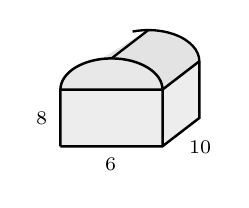
\begin{tikzpicture}[scale=0.72, every node/.style={font=\scriptsize, text=black}]
      % ហិបដែក (ប្រអប់កែង 10x6x8 + កន្លះស៊ីឡាំង r=3, h=10)
      \coordinate (A) at (-1.30,-0.75);
      \coordinate (B) at (0.50,-0.75);
      \coordinate (C) at (1.15,-0.25);
      \coordinate (A1) at (-1.30,0.25);
      \coordinate (B1) at (0.50,0.25);
      \coordinate (C1) at (1.15,0.75);
      \fill[gray!14] (A) -- (B) -- (C) -- (C1) -- (B1) -- (A1) -- cycle;
      \fill[gray!22] (B1) arc (0:180:0.90 and 0.55) -- (-0.65,0.75) -- (0.25,1.30) arc (90:0:0.90 and 0.55) -- cycle;
      \draw[black, line width=0.9pt] (A) -- (B) -- (C) -- (C1) (A) -- (A1) -- (B1) -- (B) (B1) -- (C1);
      \draw[black, line width=0.9pt, fill=gray!18] (B1) arc (0:180:0.90 and 0.55) -- cycle;
      \draw[black, line width=0.85pt] (C1) arc (0:108:0.90 and 0.55);
      \draw[black, line width=0.85pt] (-0.40,0.80) -- (0.25,1.30);
      \node[below=0.5pt] at (-0.40,-0.75) {$6$};
      \node[below right=-1pt] at (0.85,-0.52) {$10$};
      \node[left=1pt] at (-1.30,-0.25) {$8$};
    \end{tikzpicture}
  \end{minipage}
\end{tcolorbox}

\end{document}
